%%%%%%%%%%%%%%%%%%%%%%% file template.tex %%%%%%%%%%%%%%%%%%%%%%%%%
% $Id: woc_2col.tex 158 2017-01-19 23:08:23Z foley $
% $URL: https://repository.cs.ru.is/svn/template/tvd/journal/matec-woc/woc_2col.tex $
% 
% This is a template file for Web of Conferences Journal
%
% Copy it to a new file with a new name and use it as the basis
% for your article
%
% This template has been updated to match the Word Template's contents
% by Joseph T. Foley < foley AT RU dot IS >
%
%%%%%%%%%%%%%%%%%%%%%%%%%% EDP Science %%%%%%%%%%%%%%%%%%%%%%%%%%%%
%
%%%\documentclass[option]{webofc}
%%% "twocolumn" for typesetting an article in two columns format (default one column)
%
\documentclass[twocolumn]{webofc}
\usepackage[varg]{txfonts}   % Web of Conferences font
\usepackage{booktabs}
\usepackage{pgfplots}
\usepackage{array} %% needed for advanced table manipulation
%% Column types from http://tex.stackexchange.com/questions/54069/table-with-text-wrapping
\newcolumntype{L}[1]{>{\raggedright\let\newline\\\arraybackslash\hspace{0pt}}m{#1}}
\newcolumntype{C}[1]{>{\centering\let\newline\\\arraybackslash\hspace{0pt}}m{#1}}
\newcolumntype{R}[1]{>{\raggedleft\let\newline\\\arraybackslash\hspace{0pt}}m{#1}}

\graphicspath{{graphics/}{graphics/arch/}{Graphics/}{./}} % Look in these folders for graphics
%
% Put here some packages required or/and some personnal commands
%
%

\begin{filecontents}{serverloads.dat}
\end{filecontents}

\begin{document}
%
\title{Web of Conferences --- A4 paper size, two columns format}
%
% subtitle is optionnal
%
%%%\subtitle{Do you have a subtitle?\\ If so, write it here}

\author{\firstname{Isaline} \lastname{Augustino}\inst{1,3}\fnsep\thanks \and
        \firstname{Isabelle} \lastname{Houlbert}\inst{2}\and
        \firstname{Agnés} \lastname{Henri}\inst{3}
        % etc.
      }

\institute{EDP Sciences, Editorial Department, 91944 Les Ulis Cedex A, France
\and
           EDP Sciences, Production Department, 91944 Les Ulis Cedex A, France
          }

\abstract{%
  You should leave 8 mm of space above the abstract and 10 mm after the abstract.
  The heading Abstract should be typed in bold 9-point Times.
  The body of the abstract should be typed in normal 9-point Arial in a single paragraph, immediately following the heading.
  The text should be set to 1 line spacing.
  The abstract should be centred across the page, indented 17 mm from the left and right page margins and justified.
  It should not normally exceed 200 words.
}
%
\maketitle
%

FEHLT WAS IST EIN LB
WARUM RUST

\section{System Architecture and Components}

Der Systementwurf baut auf dem System \textit{Docker} auf {\color{red}HIER QUELLE ZU WAS IST DOCKER} und dem darunter liegenden System zum deployen von mehreren Container Instanzen \textit{Docker Compose}. Die Nutzung von \textit{Docker} fällt aufgrund der Verbreitung als Industriestandart {\color{red} QUELLE}.
\begin{figure}[htbp]
\centering
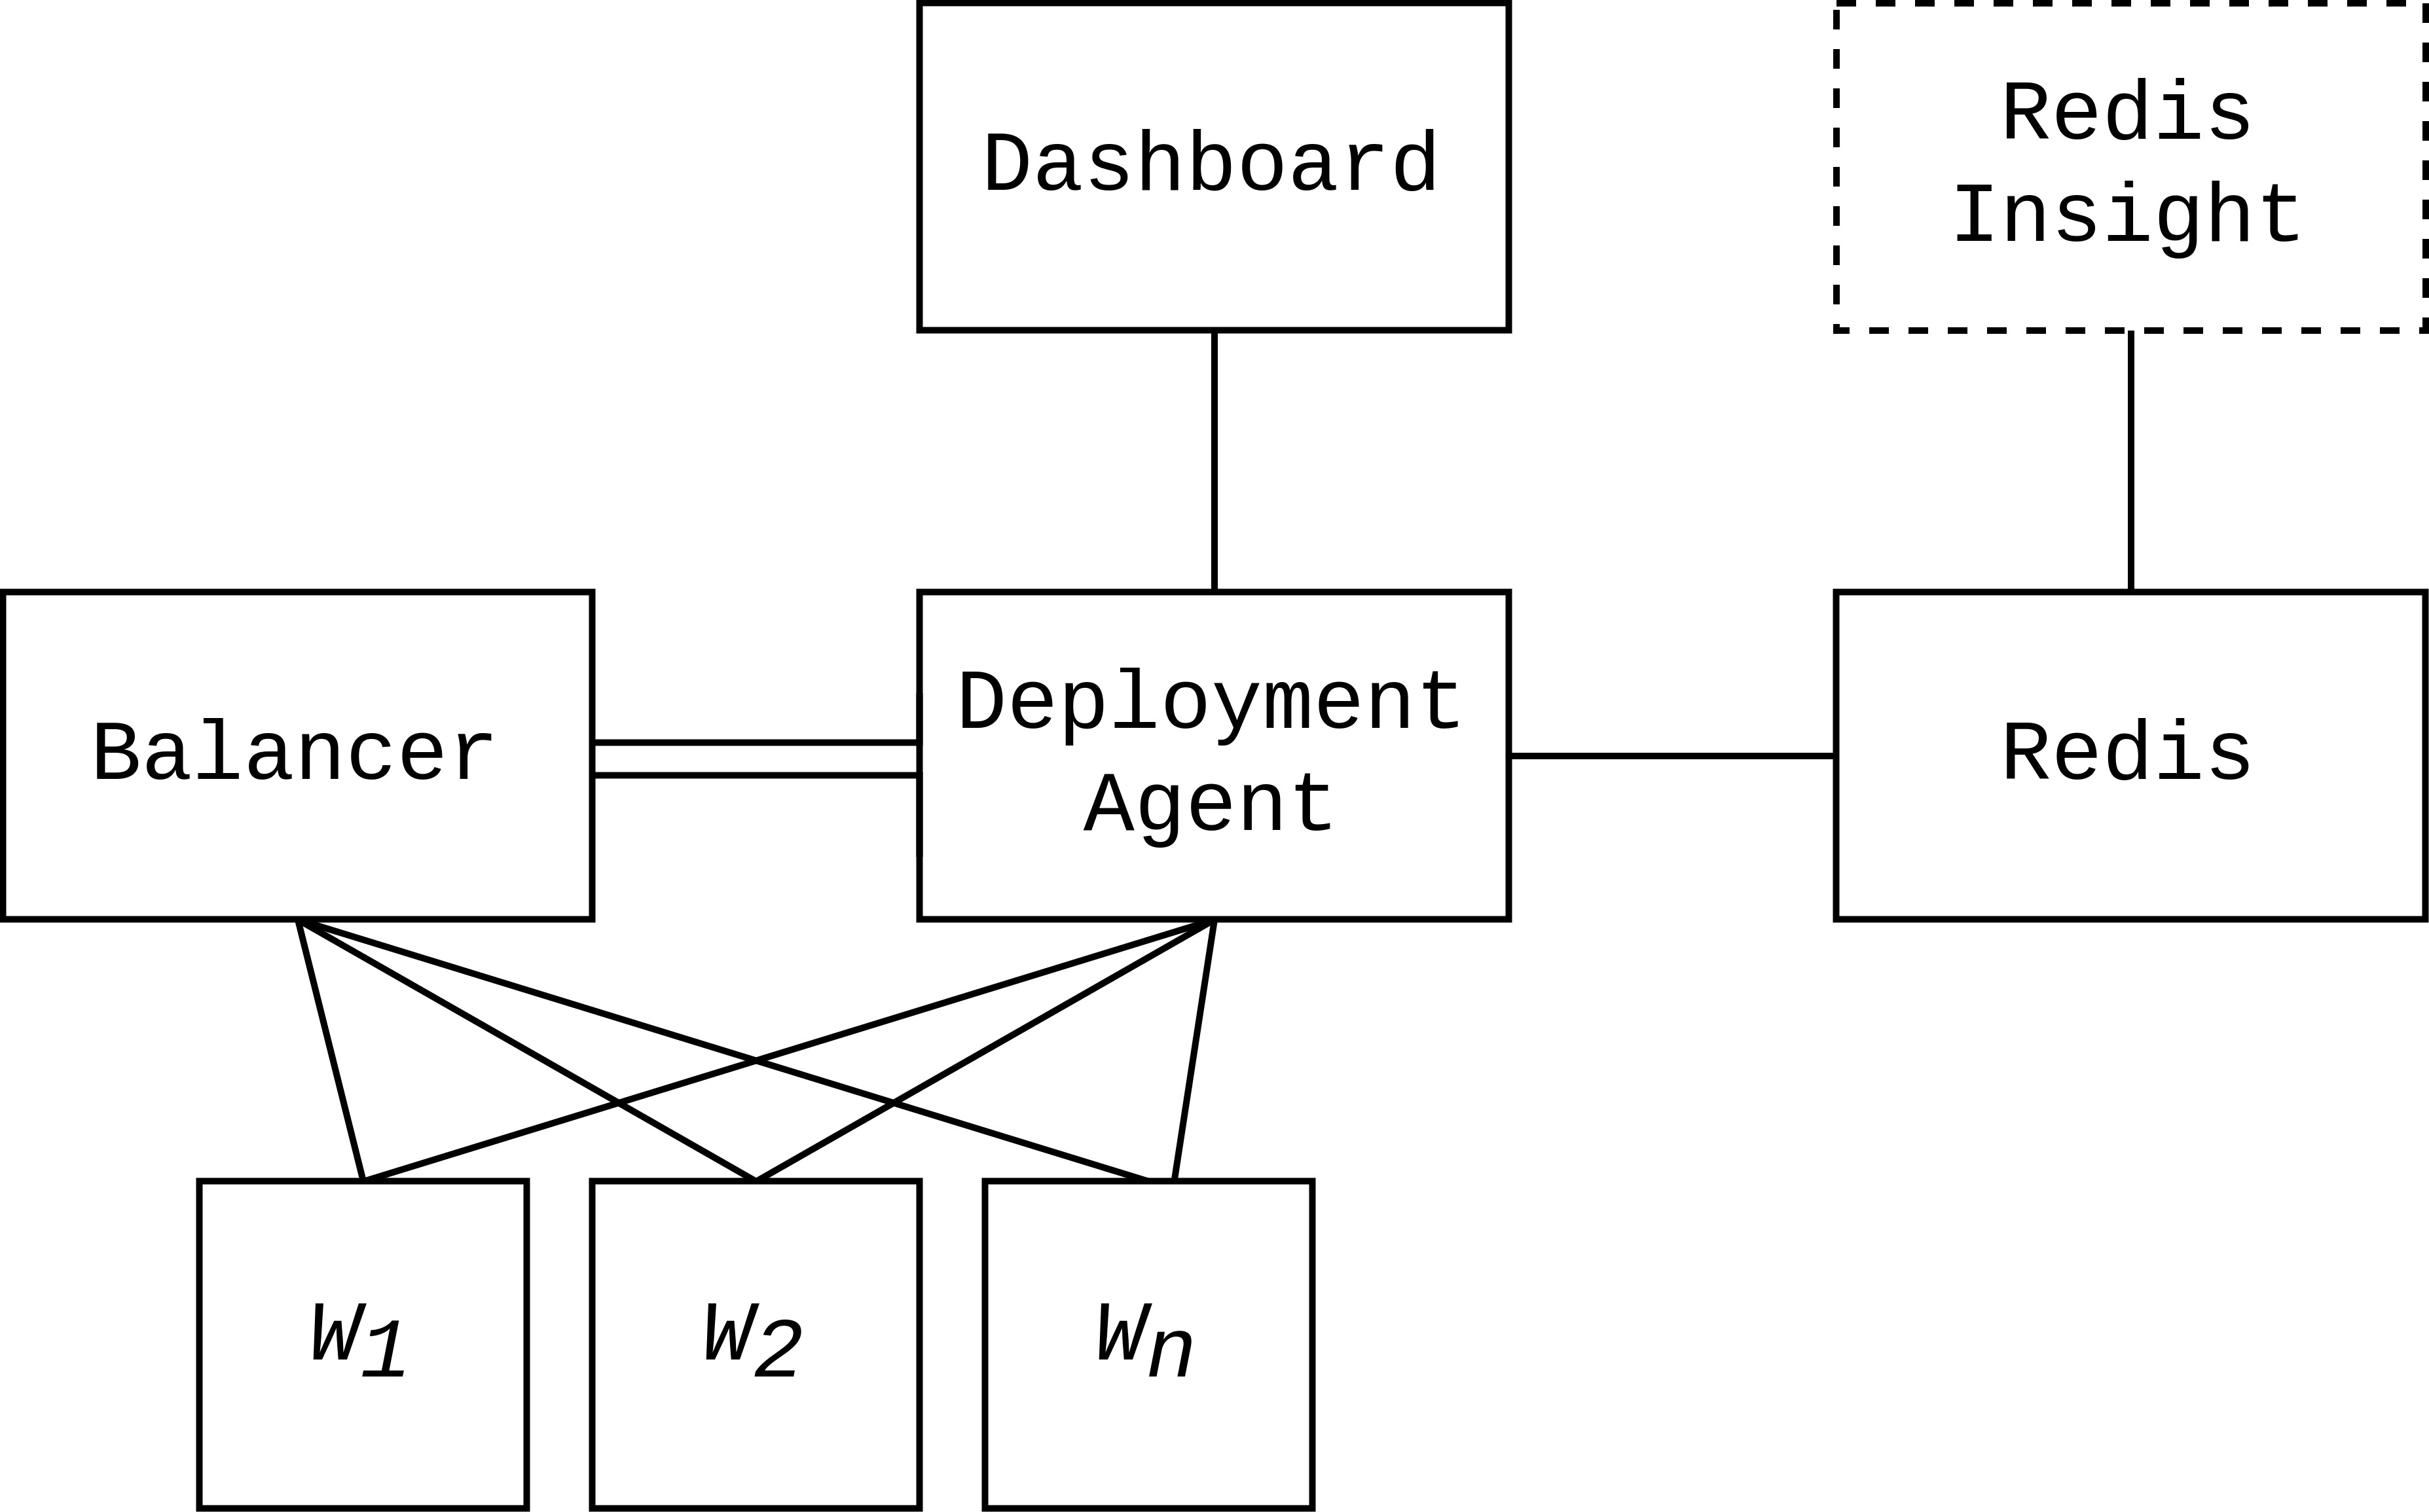
\includegraphics[width=\columnwidth]{minimaloverview.jpg}
\caption{This diagram provides a comprehensive overview of all components, each of which represents an active container within the system landscape established during the deployment process.}
\label{fig:minimal}
\end{figure}

Figure~\ref{fig:minimal} serves as the foundational framework for comprehending all subsequent elucidations. The architecture is derived from its task distribution. As one of the two core units, the \textit{Balancer} ensures the distribution of workload to the workers, while the interaction among workers occurs within the \textit{Deployment-Agent}. The latter will be addressed in detail in the following sections. The \textit{Worker} constitutes a fundamental operational unit within the system architecture, designed to receive and process distributed workload. This component is subject to scaling, with a minimum instantiation of one instance, and can be replicated up to the maximum capacity as determined by the host system's resource constraints. This scalability feature enables dynamic adjustment of processing capabilities in response to varying computational demands.
\textit{Redis} (Remote Dictionary Server), a high-performance, open-source, in-memory key-value data store {\color{red} QUELLE}, is utilized to maintain a persistent state between the currently active resources and the \textit{Workers} that are intended to be operational. This mechanism facilitates the synchronization of system state across running and desired instances, enabling efficient resource management and system consistency. When examining the connection process from the high-level perspective we currently occupy, the sequence unfolds as follows: A client initiates a request via HTTP to a specific port, which is received by the \textit{Balancer}. The \textit{Balancer} obtains information about available clients and their current utilization over a Socket from the \textit{Deployment Agent}. Subsequently, the workload is distributed in proportion to this utilization data.
Administrators and developers can access more detailed information through the \textit{Dashboard} and, optionally, \textit{Redis Insight}. It should be noted that the \textit{Dashboard} and \textit{Redis Insight} are not subjects of further discussion in this paper.
The subsequent chapters will elucidate the operational mechanisms of the components at a significantly more granular level.

\section{Verteilung der Last an die Worker}
Der Algorithmus für die Verteilung der eingehenden Fragen an die Verfügbare anzahl an Arbeitern basiert auf der Idee, dass jedes Element in einer Warteschlange ein Gewicht hat, das von einem Score abgeleitet wird. Der Score beschreibt eine Leistungsmetrik. Die Auswahl eines Elements erfolgt proportional zu seinem Gewicht. Jedes Element \( i \) hat einen Score \( s_i \). Das Gewicht \( w_i \) eines Elements ist Konfigurierbar und auf die jeweilige Ressource abzustimmen. Im Kontext der System Übersicht (siehe Figure~\ref{fig:minimal}) erfolgt die Berechnung dieses Gewichts, die Erstellung der Warteschlange und Eingliederung in diese innerhalb des \textit{Deployment Agents}, wird dann über den Socket periodisch zur Verteilung an den \textit{Balancer} übermittelt.

\subsection{Berechnung der Scores}
Ein Score \( s_i \) eines \textit{Workes} ist ein Gesamtscore verschiedener Metriken:
$$s_i = w_c \cdot s_c + w_m \cdot s_m + w_n \cdot s_n + w_a \cdot s_a$$
Dabei ist dieser Gesamtscore zusammengesetzt aus Socres einzelnenr Disziplinen und gewichten ( \( W_C, W_M, ... \)). Die  \( CPU_{usage} \) eines \textit{Workers} ergibt sich durch:
$$CPU_{usage} = \frac{\Delta CPU}{\Delta System} \cdot N_{CPU} \cdot 100\%$$
Wobei das Delta sich aus der Differenz der CPU-Nutzung zwischen zwei Messzeitpunkten und Differenz der System-CPU-Nutzung zwischen zwei Messzeitpunkten under der Berücksichtigung der Anzahl an Kernen ergibt. Recht ähnlich dazu ergibt sich die Speicherauslastung:
$$Memory_{usage} = \frac{Memory_{used}}{Memory_{limit}} \cdot 100\%$$
Hier wird die Speichernutzung wird als Prozentsatz des genutzten Speichers im Verhältnis zum Limit berechnet. Die Netzwerknutzung wird basierend auf der Änderung des Datenverkehrs über die Zeit berechnet:
$$Network_{usage} = \frac{\Delta Bytes_{total}}{t \cdot 10^6} \text{ MB/s}$$
Dabei wird die Gesamtänderung der übertragenen Bytes (Empfangen + Gesendet)
durch die Zeitdifferenz zwischen den Messungen in Sekunden genommen. Die prozentuale Netzwerknutzung wird dann als relative Änderung zur vorherigen Messung berechnet:
$$Network_{usage\%} = \left(\frac{Network_{usage} - Network_{usage_{prev}}}{Network_{usage_{prev}}}\right) \cdot 100\%$$
Am schwierigsten gestalte sich die letzte Metrik der Verfügbarkeit. Da der Inhalt, welcher am Ende innerhalb der \textit{Worker} läuft am Ende selbstverständlich variabel ist gibt es keinen fixen Wert ab dem man sagen könnte dass ein Container schnell ist bzw. eine hohe Verfügbarkeit aufweißt. Um sich nun einer Verfügbarkeitswertung anzunähren braucht es neben einen Basiswert aus Antwortzeiten. Dieser Setzt sich wie folgt zusammen:
$$Score_{base} = 100 \cdot \left(\frac{BestTime}{EffectiveTime}\right)^{1.5}$$
Wobei die \( EffectiveTime = 0.3 \cdot CurrentTime + 0.7 \cdot AvgTim \), die \( BestTime \) ist die  Durchschnitt der besten Antwortzeiten. \( AvgTime \) die Durchschnittliche Antwortzeit. Ein Strafterm wird für die Verfügbarkeit angewendet, wenn die effektive Zeit den dynamischen Schwellenwert überschreitet:
$$Penalty = 20 \cdot (1 - e^{-(EffectiveTime - Threshold)})$$
Eines der wichtigsten Schritte in diesem prozess kommt dann mit der Trendanpassung.
Eine Trendanpassung wird basierend auf der jüngsten Entwicklung der Antwortzeiten vorgenommen:
$$Trend = \frac{AvgTime_{older} - AvgTime_{recent}}{AvgTime_{older}}$$
$$TrendAdjustment = Trend \cdot 10$$
Um alle Werte Final in den Verfügbarkeits Score zu überführen muss dann:
$$S_A = \max(0, \min(100, Score_{base} - Penalty + TrendAdj.))$$ Alle Gewichte werden gegengerechnet am Ende gegen Gerechnet mit \( S_X = 100\% - Y_{usage} \), dadurch ergibt sich dass 100 insgesamt aber auch pro Score das beste ist Ergebnis ist. 

\subsection{Verteilung der Scores}
The \textit{Balancer} requires the scores to effectively distribute load according to corresponding utilization. For communication via the socket, a queue is implemented. In information technology, a queue possesses the essential characteristic of determining order based on the First In, First Out principle {\color{red} SOURCE}. In the context of the described load balancer, the queue \( Q \) represents an ordered data structure comprising elements \( (Q_i, s_i) \), where \( Q_i \) denotes the element and \( s_i \) its associated score. This queue exhibits a dynamic size, allowing it to accommodate any number of elements as needed. Formally, we can define a queue as a set:
$$Q = \{ (Q_1, s_1), (Q_2, s_2), \dots, (Q_n, s_n) \}, \quad n \in \mathbb{N}$$
In this representation, \( n \) signifies the number of elements within the queue, which can grow arbitrarily large. The queue undergoes both periodic generation and querying processes. The queue grows as the system, specifically the \textit{Deployment-Agent}, scales multiple containers, thereby altering the pairs within the queue. Theoretically, a queue can contain an infinite number of \textit{Workers}, although in practice, system resources limit its size. In practical implementation, the queue within the Load Balancer initializes and contracts to the configured default number of \textit{Workers}, and scales up to the configured upper limit. Additionally, in the actual implementation, the queue also sends the utilization category for each container, derived from the calculated score \( s_i \). This category will be explained in the next subchapter.

\subsection{Zustände eines \textit{Workers}}
The algorithmic approach involves transforming numerical scores into utilization categories, a process designed to enhance interpretability. This reduction of continuous scores into discrete categories (Low, Medium, High Utilization) significantly eases data interpretation. This approach is grounded in the psychological principle of cognitive load, which posits that humans more readily process and comprehend discrete categories compared to continuous values {\color{red} SOURCE}. Moreover, this categorization method offers an inherent buffer against minor measurement fluctuations, providing a degree of error tolerance in the analysis.
\begin{figure*}[htbp]
\centering
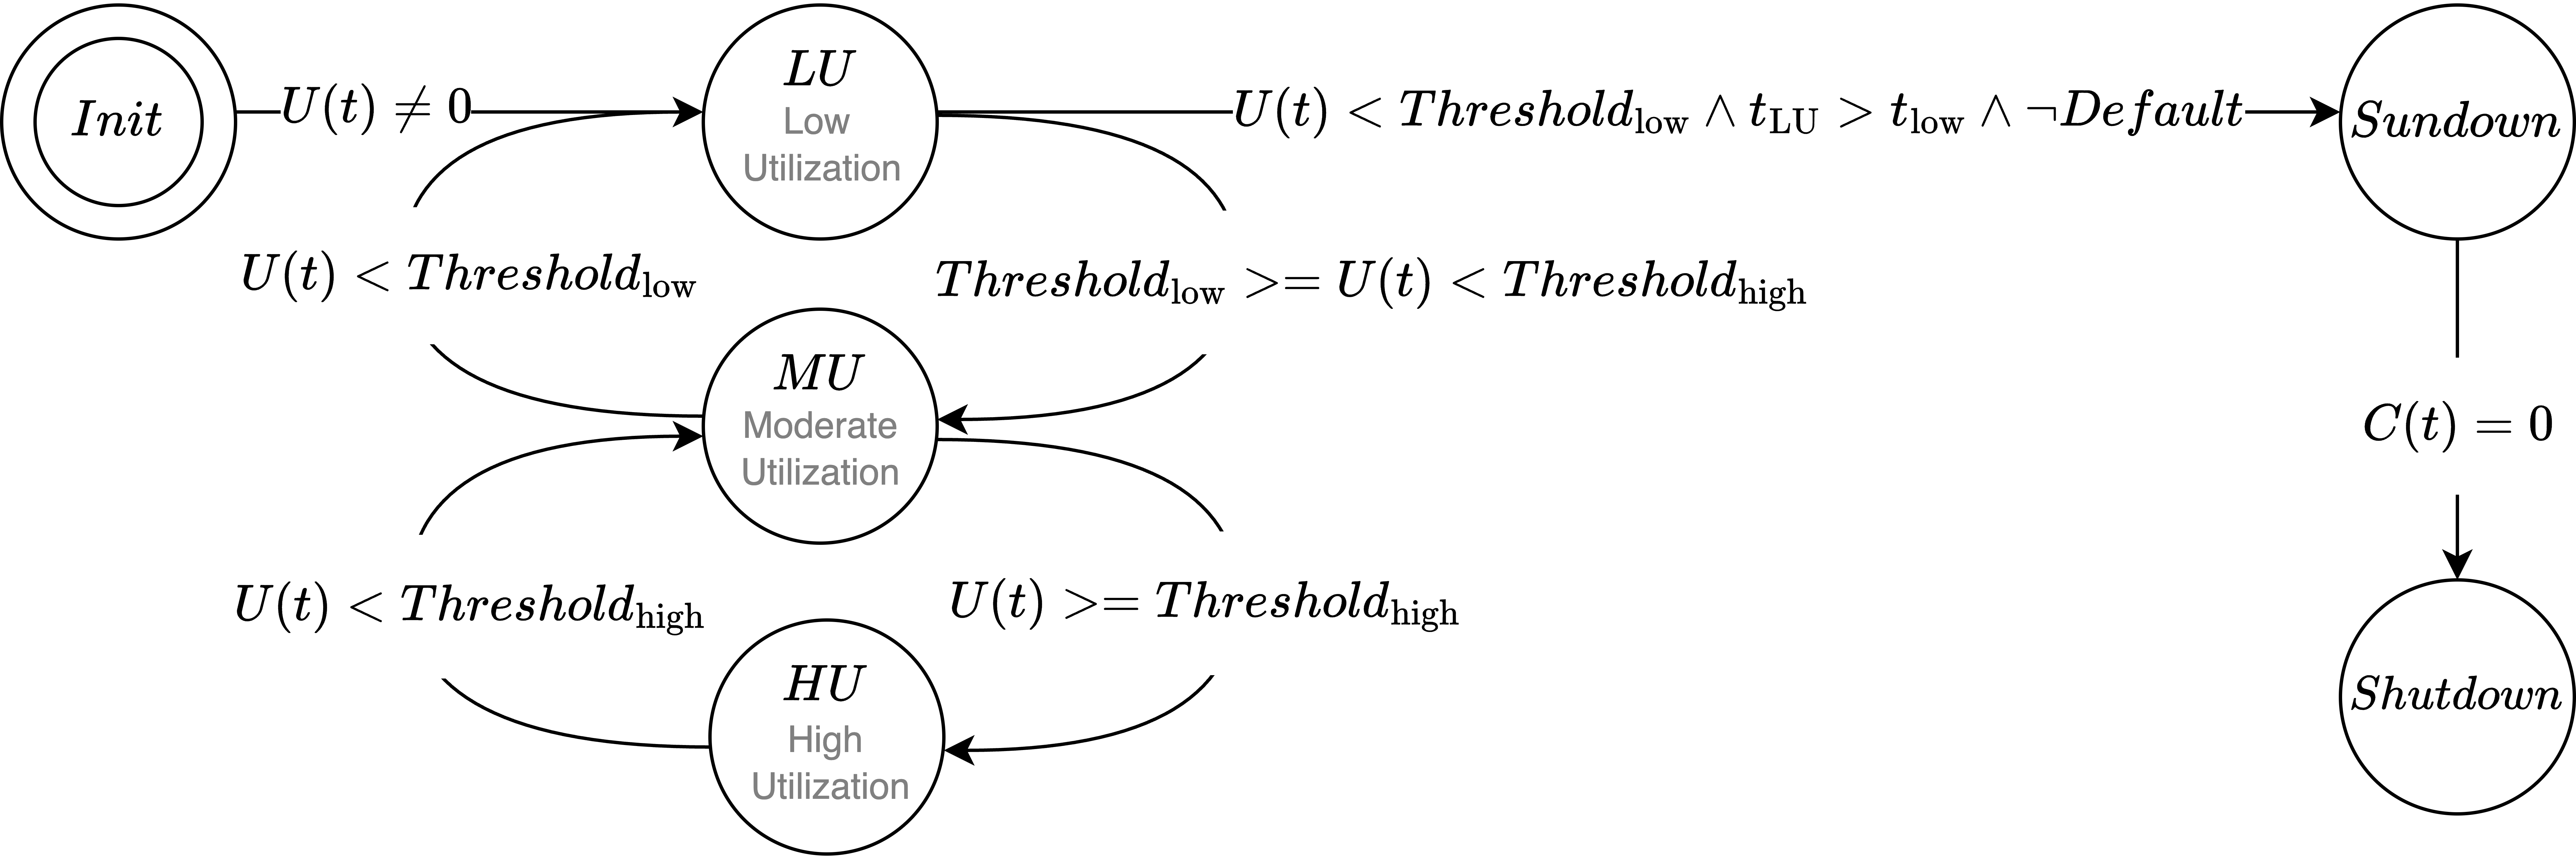
\includegraphics[width=\textwidth]{utilizations.drawio.png}
\caption{Finite state automaton illustrating worker state transitions based on workload levels. Transitions are governed by thresholds $Threshold_{low}$ and $Threshold_{high}$, with a hysteresis mechanism to prevent unnecessary reallocations. The final shutdown occurs when active connections $C(t)$ reach zero.}
\label{fig:automat}
\end{figure*} The algorithm for the transition between the states of a \textit{worker} can be explained using the finite automaton depicted in Figure~\ref{fig:automat}. The presented model is based on a stochastic finite automaton representing different workload levels. The state transitions are controlled by a multidimensional evaluation function, whose thresholds $Threshold_{low}$ and $Threshold_{high}$ are based on empirical data from large cloud providers {\color{red} SOURCE}, but can also be modified in the application configuration afterward. A central element of the model is the Sundown state, defined by \( P(LU \rightarrow Sundown) \) as:
$$P(U(t) < Threshold_{low} \wedge t_{LU} > t_{low} \wedge \neg Default) $$
This state implements a hysteresis mechanism that distinguishes short-term load fluctuations from long-term trends, thus preventing unnecessary resource reallocations. The transition to the final shutdown state is governed by the condition $C(t) = 0$, where $C(t)$ represents the cardinality of the set of active connections at time $t$. The differentiation between default and non-default workers leads to a conditional termination property:

$$ \forall w \in W: T(w) = \begin{cases} 
0 & \text{if } w \in D \\
1 & \text{if } w \notin D
\end{cases} $$

Here, $W$ represents the set of all workers, $D \subset W$ the subset of default workers, and $T(w)$ the termination function. This distinction enables fine-grained control over system stability and scalability. The model addresses the challenges of dynamic load balancing in microservice architectures and provides a theoretical framework for implementing adaptive orchestration strategies. Elements of queueing theory are applied in the analysis of connection states and resource request management, particularly where the consideration of $C(t)$ shows parallels to M/M/c queueing models {\color{red} SOURCE}. Additionally, it integrates aspects of the Markov decision process, especially in the modeling of state transitions, allowing a probabilistic view of the system dynamics {\color{red} SOURCE}. This enables the system to maintain an optimal balance between resource efficiency and service availability. The consideration of connection states and worker classification allows for fine-grained control over resource allocation, which is particularly important in highly scalable, containerized infrastructures.

\subsection{Scaling}  
Building on the finite automatom previously introduced (Figure~\ref{fig:automat}), the process of scaling containers up and down can now be described. The system’s decision to launch a new \textit{worker} is modeled by state transitions, which are triggered by predefined threshold values. These transitions are governed by configurable variables. Specifically, \( C_{\text{running}}(t) \) denotes the number of active containers at time \( t \), while \( C_{\text{default}} \) represents the minimum predefined number of containers, and \( C_{\text{max}} \) represents the maximum allowable number of containers. Both values are configurable. As previously discussed, \( U(t) \) represents the system utilization at time \( t \), which is calculated based on the corresponding performance scores.

\subsubsection{Scale-up (container start-up)}
The process of scaling up new containers is triggered when the current number of running containers \( C_{\text{running}}(t) \) falls below the predefined threshold and the system utilization \( U(t) \) exceeds a critical threshold \( U_{\text{critical}} \). This critical threshold is also configurable and must be adjusted by the administrator according to the resources distributed across the workers. The conditions for scaling up can be summarized as follows:
\[
C_{\text{running}}(t) < C_{\text{default}}, \quad U(t) \geq U_{\text{critical}}
\]
Once these conditions are met, the number of running containers is incremented:
\[
C_{\text{running}}(t+1) = C_{\text{running}}(t) + 1
\]
This implies that the number of containers is increased by one when the specified conditions hold.

\subsubsection{Scale-down (container shutdown)}
The process of scaling down containers is initiated when the system utilization falls below a defined threshold \( U_{\text{low}} \), while the number of running containers \( C_{\text{running}}(t) \) exceeds the minimum required number \( C_{\text{default}} \). Transitioning to a "scale-down" state is essential because containers (or \textit{workers}) cannot be immediately shut down—they may still hold tasks in the queue, or even if not in the queue, they could maintain active connections. It is crucial to ensure that there is a state where old connections are still functional, but no new ones are accepted. The conditions for scaling down are met when:
\[
C_{\text{running}}(t+1) = \max(C_{\text{default}}, C_{\text{running}}(t) - R)
\]
where \( R \) represents the number of containers that are scaled down in a single step, which depends on the current utilization and the load management policies specified in the configuration.

\subsubsection{Cooldown Periods}
In addition to the above conditions, a cooldown period \( T_{\text{cooldown}} \) is defined to ensure that a minimum amount of time \( t_{\text{elapsed}} \) has passed between two scaling actions. This condition can be expressed as:
\[
t_{\text{elapsed}} \geq T_{\text{cooldown}}
\]
During the cooldown period, no scale-up or scale-down actions are performed, thereby preventing excessive start-stop cycles that could negatively impact system stability.

\subsection{Lastverteilungsmodell}
Der Dynamic Weighted Load Balancer basiert auf dem Prinzip der gewichteten Zufallsauswahl, die durch eine diskrete Wahrscheinlichkeitsverteilung modelliert wird. Sei \( \mathcal{S} = \{s_1, \ldots, s_N\} \) die Menge der verfügbaren Server und \( \mathcal{W} = \{w_1, \ldots, w_N\} \) die entsprechenden Gewichte. Die Wahrscheinlichkeit \(  p_i \), dass Server \( s_i \) ausgewählt wird, ist definiert als:
$$
p_i = \frac{w_i}{\sum_{j=1}^N w_j}, \quad i = 1, \ldots, N
$$
Diese Verteilung entspricht einer kategorischen Verteilung mit Parameter \(\mathf{p} = (p_1, \ldots, p_N)\). Für das Lastenmodell gilt dann, es sei \(R\) die Gesamtzahl der Anfragen. Die erwartete Anzahl der Anfragen \(r_i\) für Server \(s_i\) folgt der Verteilung \( (r_1, \ldots, r_N) \sim \text{Multinomial}(R, \mathf{p}) \) mit dem theoretischen Erwartungswert von:
$$
\mathbb{E}[r_i] = R \cdot p_i = R \cdot \frac{w_i}{\sum_{j=1}^N w_j}
$$
Um nun die Effizienz dieser Verteilung beurteilen zu können werden zwei Szenarien vergleichen. Zur Gegenüberstellung dient die folgende Effiziensmetrik, diese Definiert die Effizienz \(\eta\):
$$
\eta = \frac{\min_{i} \{r_i / w_i\}}{\max_{i} \{r_i / w_i\}}
$$
Wir untersuchen zwei kontrastierende Szenarien mit \(N = 4\) Servern und \(R = 10^4\) Anfragen

\subsubsection{Approximation of Heterogeneous Loads}
Bei einer Auslastung von \(\mathcal{W}_1 = \{100, 50, 25, 5\}\) ergibt sich eine theoretische Lastenverteilung von \( \mathbb{E}[r_i] = (5556, 2778, 1389, 278)\). Bei einer simulierten Verteilung von \((5600, 2700, 1400, 300)\) erhalten wir: 

$$\eta_1 = \frac{\min \{56, 54, 56, 60\}}{\max \{56, 54, 56, 60\}} = 0.9$$

\subsubsection{Annäherung einer Homogene Auslastungen}
Bei einer ausgeglicheneren Auslastung von \(\mathcal{W}_2 = \{100, 95, 90, 85\}\) liegt die theoretische Verteilung bei \(\mathbb{E}[r_i] = (2700, 2570, 2430, 2300)\) Bei einer Simulierten Verteilung ergibt sich:
$$
\eta_2 = \frac{\min \{27.2, 26.84, 27.22, 26.82\}}{\max \{27.2, 26.84, 27.22, 26.82\}} \approx 0.985
$$

\subsubsection{Measurement Data Collection}
In order to empirically validate the theoretical framework, measurement data was collected based on the \textit{workers}, scores, and utilization categories. The programmatic components for calculating the weights based on the probability model were implemented using a function that generated random queues. The execution cycle of the program first instantiated a queue, calculated the weights based on the random scores, and subsequently updated the statistics of the \textit{workers} for the following iteration. It is important to note that this data collection method represents a worst-case scenario for heterogeneous utilization, as the fluctuation range of incoming queues per time-based distribution iteration is significantly more varied in real-world conditions. The script used for generating the measurement data was executed 100 times, with minor delays introduced between each simulation run. The simulation itself, similar to the actual implementation, adhered to identical temporal intervals. 

\subsubsection{Interpretation}
The analysis demonstrates that the Dynamic Weighted Load Balancer achieves high efficiency in both theoretical scenarios. In the heterogeneous case (\(\eta_1 = 0.9\)), despite significantly varying server capacities, an almost optimal relative load distribution is achieved. In the homogeneous case (\(\eta_2 \approx 0.985\)), efficiency approaches the theoretical maximum of 1. As for the evaluation of the collected data, it can initially be examined in the following time series. Based on this graphical evaluation, the measured data can be considered valid. Each graph exemplifies a single \textit{worker}. The weights are updated based on a new queue at times \(t=2\), \(t=4\), and so on. What is particularly noticeable is how, after a period of high load for a \textit{worker}, the probability of being assigned new loads decreases significantly when utilization exceeds \(50\%\), allowing the \textit{worker's} load to recover swiftly. This recovery ensures that the \textit{worker} is ready and available for new loads in the next cycle.
\begin{figure}[htbp]
\centering
\begin{tikzpicture}
\begin{axis}[
    width=\columnwidth,
    height=7cm,
    xlabel={Zeit},
    ylabel={Auslastung (\%)},
    ylabel style={at={(axis description cs:0.1,.5)}, anchor=south},
    xmin=0, xmax=33.5,
    ymin=0, ymax=65,
    xtick distance=5,
    ytick distance=10,
    grid=major,
    cycle list name=color list,
]

\addplot[thick] table[x index=0, y index=1, col sep=tab] {data.txt};
\addplot[thick] table[x index=0, y index=2, col sep=tab] {data.txt};
\addplot[thick] table[x index=0, y index=3, col sep=tab] {data.txt};
\addplot[thick] table[x index=0, y index=4, col sep=tab] {data.txt};
\end{axis}
\end{tikzpicture}
\end{figure}
Further interpretation reveals that the load oscillates around the theoretical ideal state. A perfect load distribution would be characterized by a constant straight line, ideally as low as possible on the Y-axis. However, this ideal state is unattainable due to the various variables and environmental factors involved. Each \textit{worker} handles a variable load—code on which the load can be distributed. These requests differ in nature. We can distinguish between human-generated requests, such as a person (user \(w\)) accessing a webpage or service \(x\), and machine-generated requests, where server \(y\) calls server \(z\). Both types of requests share a common feature: the variability in the nature of the requests inherently causes the workers' utilization to fluctuate, for example, due to differing payloads. Additional external factors, such as network speed, contribute to these fluctuations. The variability is even greater with human-generated requests, as they can be interrupted at unpredictable times. All of these factors make a linear distribution impossible. Consequently, load distribution that adapts to varying loads necessarily results in oscillations. This partially answers the question as to why such overhead in load balancing is justified. A comparison with a traditional round-robin algorithm, which introduces virtually no overhead {\color{red} SOURCE}, reveals that in an ideal scenario—where requests arrive at regular intervals, finish simultaneously, have identical payloads, and all participants are equally available—round-robin would indeed result in perfect load distribution. However, as previously discussed, real-world conditions deviate significantly from this ideal. In a worst-case scenario, a worker with extremely high utilization could coexist alongside another worker with almost no utilization, yet both would receive the same load. This justifies the overhead introduced by dynamic load balancing, as it enables the system to continuously adapt and recalibrate, regardless of how extreme or uncertain the incoming requests may be.

\section{Cache}
Der Fokus dieser Arbeit ist klar im Verbund ein Loadbalancing mit dynamsicher lastenverteilung und Autoskalierung performant zu implementieren. Gerade in der Disziplin der Performance spielt Caching eine erhebliche rolle ist aber Komplex {\color{red} SOURCE}. Unterschieden wird in statisches und Dynamsches caching. Das dynamische Caching verändert das Caching-Modell vollständig und ermöglicht die Zwischenspeicherung einer viel breiteren Palette von Inhalten, einschließlich hochdynamischer Webseiten {\color{red} SOURCE}. Im beschriebenen System wird ein minimalistischerer statischer Cache verwendet, der Einträge speichert, um die Latenz für häufig angeforderte Daten zu verringern und die Anzahl der Backend-Abfragen zu reduzieren. Der Cache ist so konzipiert, dass er eine vorgegebene Kapazität hat und Einträge basierend auf ihrer Verfallszeit (TTL) entfernt werden. Diese Implementierung trägt dazu bei, die Effizienz des Systems zu erhöhen, indem alte oder selten genutzte Daten automatisch gelöscht werden. Der Cache basiert auf der \textit{Rust} Datenstruktur \texttt{VecDeque}, einer doppelten Warteschlange, die es ermöglicht, sowohl Einträge am Anfang als auch am Ende in O(1)-Zeit hinzuzufügen oder zu entfernen {\color{red} SOURCE}. Dies ist besonders nützlich, wenn der Cache seine Kapazität erreicht und der älteste Eintrag entfernt werden muss. Die Cache-Einträge bestehen aus drei Komponenten:  dem Schlüssel \( k_i \), der zu speichernde Cache Wert \( v_i \) und dem Verfallssdatum \( t_i \). Wir definieren den Cache formal als eine Menge \( C \), die \( N \) Einträge enthält:
\[
C = \{ (k_1, v_1, t_1), (k_2, v_2, t_2), \dots, (k_N, v_N, t_N) \}
\]
Der Cache arbeitet mit einer TTL (Time-to-Live)-Strategie, bei der jeder Eintrag \( (k_i, v_i, t_i) \) nur so lange im Cache verbleibt, bis \( t_i \), der Verfallszeitpunkt, erreicht ist. Ist die aktuelle Zeit \( t_{\text{now}} \) größer als \( t_i \), wird der Eintrag entfernt. Um verfallene Einträge zu entfernen, enthält der Cache eine Garbage Collection, die regelmäßig in einem Hintergrundprozess läuft. Dieser Prozess überprüft alle Einträge in bestimmten Zeitintervallen \( \Delta t \), um veraltete Einträge zu entfernen und den Speicher effizient zu nutzen.

\subsection{Zugriffsoperationen}
Beim Abrufen eines Wertes aus dem Cache wird geprüft, ob der Eintrag noch gültig ist. Ist der Eintrag abgelaufen, wird er entfernt, und der Cache gibt \texttt{none} zurück. Andernfalls wird der zwischengespeicherte Wert zurückgegeben. Beim Speichern eines neuen Eintrags wird zunächst überprüft, ob der Cache voll ist. Falls dies der Fall ist, wird der älteste Eintrag entfernt, bevor der neue Eintrag hinzugefügt wird.

\subsection{Auswirkungen auf die Systemleistung}
Der Cache reduziert die Anzahl der Backend-Anfragen und optimiert die Ressourcennutzung. Die Trefferquote (Hit Rate) \( H \) beschreibt den Anteil der Anfragen, die direkt im Cache beantwortet werden können:

\[
H = \frac{N_{\text{hit}}}{N_{\text{total}}}
\]

Eine höhere Trefferquote führt zu einer verbesserten Gesamtleistung des Systems, da weniger Anfragen weitergeleitet werden müssen. Gleichzeitig minimiert der Cache die Latenz bei der Beantwortung von Anfragen, was besonders in hochgradig skalierbaren Umgebungen entscheidend ist {\color{red} SOURCE}.

\section{Anfragenmanagement}



\bibliography{references}





\end{document}

% end of file template.tex
%%%%%%%%%%%%%%%%%%%% TeXStudio Magic Comments %%%%%%%%%%%%%%%%%%%%%
%% These comments that start with "!TeX" modify the way TeXStudio works
%% For details see http://texstudio.sourceforge.net/manual/current/usermanual_en.html   Section 4.10
%%
%% What encoding is the file in?
% !TeX encoding = UTF-8
%% What language should it be spellchecked?
% !TeX spellcheck = en_US
%% What program should I compile this document with?
% !TeX program = pdflatex
%% Which program should be used for generating the bibliography?
% !TeX TXS-program:bibliography = txs:///bibtex
%% This also sets the bibliography program for TeXShop and TeXWorks
% !BIB program = bibtex

%%% Local Variables:
%%% mode: latex
%%% TeX-master: t
%%% End:
